% Requires: \usepackage{tikz,float}  \usetikzlibrary{arrows.meta,positioning,calc,shapes.geometric}
% Compile with pdflatex (or xelatex/lualatex for direct UTF-8 accents).
\documentclass[tikz,border=10pt]{standalone}
\usepackage[utf8]{inputenc}
\usepackage[T1]{fontenc}
\usepackage{float}
\usetikzlibrary{arrows.meta,positioning,calc,shapes.geometric}

\tikzset{
  hist/.style={rectangle, rounded corners=3pt, draw=blue!55!black, thick,
    fill=blue!8, font=\footnotesize, align=center, text width=4.8cm, inner sep=6pt},
  new/.style={rectangle, rounded corners=3pt, draw=orange!70!black, thick,
    fill=orange!10, font=\footnotesize, align=center, text width=4.8cm, inner sep=6pt},
  decision/.style={diamond, draw=black, thick, fill=yellow!10, aspect=2.4,
    font=\bfseries\footnotesize, align=center, text width=2.7cm, inner sep=2pt},
  branchblue/.style={rectangle, rounded corners=3pt, draw=blue!55!black, thick,
    fill=blue!10, font=\footnotesize, align=center, text width=3.6cm, inner sep=6pt},
  branchorange/.style={rectangle, rounded corners=3pt, draw=orange!70!black, thick,
    fill=orange!12, font=\footnotesize, align=center, text width=3.6cm, inner sep=6pt},
  branchgray/.style={rectangle, rounded corners=3pt, draw=black!55, thick,
    fill=black!5, font=\footnotesize, align=center, text width=3.6cm, inner sep=6pt},
  outbox/.style={rectangle, rounded corners=3pt, draw=black!70, very thick,
    fill=black!8, font=\bfseries\footnotesize, align=center, text width=6.6cm, inner sep=7pt},
  notebox/.style={rectangle, rounded corners=4pt, draw=black!50, dashed, thick,
    fill=yellow!8, font=\footnotesize, align=left, text width=13.5cm, inner sep=8pt},
  arrH/.style={-{Latex[length=2.2mm]}, thick, blue!55!black},
  arrN/.style={-{Latex[length=2.2mm]}, thick, orange!70!black},
  arrG/.style={-{Latex[length=2.2mm]}, thick, black!60},
}

\begin{document}
\begin{figure}[H]
\centering
\small
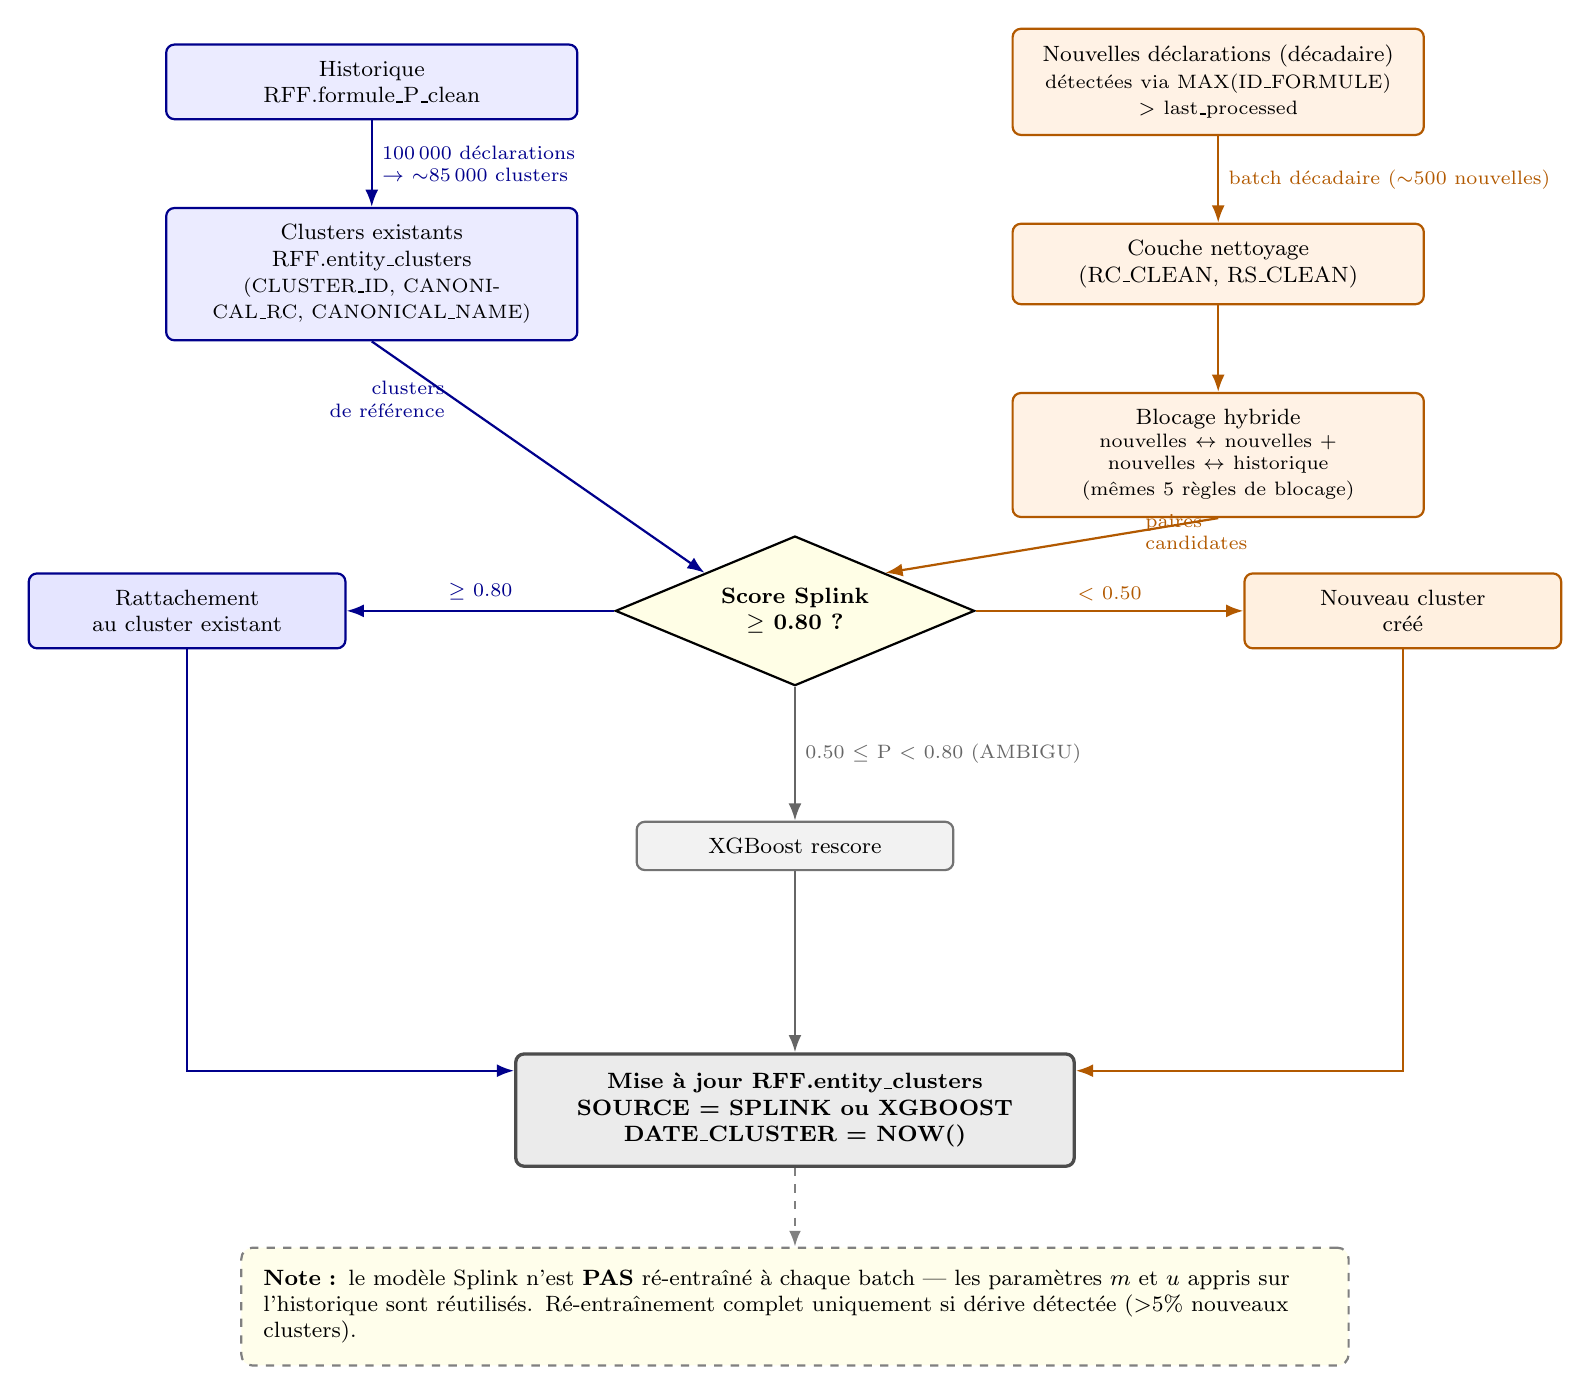
\begin{tikzpicture}[node distance=1.1cm]

% ================= LEFT TRACK : HISTORIQUE (bleu) =================
\node[hist] (l1) {Historique\\RFF.formule\_P\_clean};
\node[hist, below=of l1] (l2)
  {Clusters existants\\RFF.entity\_clusters\\
   \scriptsize(CLUSTER\_ID, CANONICAL\_RC, CANONICAL\_NAME)};

% ================= RIGHT TRACK : NOUVELLES DÉCLARATIONS (orange) =================
\node[new, right=5.5cm of l1] (r1)
  {Nouvelles déclarations (décadaire)\\
   \scriptsize détectées via MAX(ID\_FORMULE) $>$ last\_processed};
\node[new, below=of r1] (r2)
  {Couche nettoyage\\(RC\_CLEAN, RS\_CLEAN)};
\node[new, below=of r2] (r3)
  {Blocage hybride\\
   \scriptsize nouvelles $\leftrightarrow$ nouvelles + nouvelles $\leftrightarrow$ historique\\
   \scriptsize (mêmes 5 règles de blocage)};

% ================= MERGE POINT =================
\node[decision] (dec) at ($(l2.south)!0.5!(r3.south)+(0,-2.3)$)
  {Score Splink\\$\geq$ 0.80 ?};

\node[branchblue,   left=3.4cm of dec]  (yes)  {Rattachement\\au cluster existant};
\node[branchgray,   below=1.7cm of dec] (amb)  {XGBoost rescore};
\node[branchorange, right=3.4cm of dec] (no)   {Nouveau cluster\\créé};

\node[outbox, below=2.3cm of amb] (out)
  {Mise à jour RFF.entity\_clusters\\
   SOURCE = SPLINK ou XGBOOST\\
   DATE\_CLUSTER = NOW()};

% ================= NOTE BOX =================
\node[notebox, below=1.0cm of out] (note)
  {\textbf{Note :} le modèle Splink n'est \textbf{PAS} ré-entraîné à chaque batch ---
   les paramètres $m$ et $u$ appris sur l'historique sont réutilisés.
   Ré-entraînement complet uniquement si dérive détectée ($>$5\% nouveaux clusters).};

% ================= ARROWS =================
\draw[arrH] (l1) -- (l2)
  node[midway, right, font=\scriptsize, align=left] {100\,000 déclarations\\$\rightarrow$ $\sim$85\,000 clusters};
\draw[arrN] (r1) -- (r2)
  node[midway, right, font=\scriptsize] {batch décadaire ($\sim$500 nouvelles)};
\draw[arrN] (r2) -- (r3);

\draw[arrH] (l2.south) -- (dec.north west)
  node[near start, left, font=\scriptsize, align=right] {clusters\\de référence};
\draw[arrN] (r3.south) -- (dec.north east)
  node[near start, right, font=\scriptsize, align=left] {paires\\candidates};

\draw[arrH] (dec.west) -- (yes.east) node[midway, above, font=\scriptsize] {$\geq$ 0.80};
\draw[arrG] (dec.south) -- (amb.north)
  node[midway, right, font=\scriptsize] {0.50 $\le$ P $<$ 0.80 (AMBIGU)};
\draw[arrN] (dec.east) -- (no.west) node[midway, above, font=\scriptsize] {$<$ 0.50};

\draw[arrH] (yes.south) |- ($(out.west)+(0,0.5)$);
\draw[arrG] (amb) -- (out);
\draw[arrN] (no.south) |- ($(out.east)+(0,0.5)$);

\draw[-{Latex[length=2mm]}, thick, black!50, dashed] (out.south) -- (note.north);

\end{tikzpicture}
\caption{Mode de traitement incrémental du pipeline de résolution d'entités --- Office des Changes.}
\label{fig:er-incremental}
\end{figure}
\end{document}
